
We begin the ``modern'' age of computer question answering and the rise of
\abr{ai} with \watson{}: an \abr{ibm}-built \abr{ai} that could play the
American game show \jeopardyf{}

It's been over a decade since \watson{} appeared on \abr{tv}, but it was
revolutionary.  This chapter will talk about how it changed my life, how it
changed the way the public thought about \abr{ai}, and how its technology
paved the way for ``modern'' \abr{ai} as exemplified by \mm{}s like \abr{gpt}.

But this isn't a love letter to \watson{}.  For all the fame and glory it won, the
\watson{} story isn't without problems.  Indeed, this chapter will make the
argument that the game was subtly rigged in a way that set back research on
\abr{ai}.

\section{Why \abr{ibm} Chose \jeopardy{} for a Grand Challenge}

\watson{} is part of a long history of ``grand challenge'' projects meant to
symbolize progress on \abr{ai}.
%
\abr{ibm} (International Business Machines) is a New York-based technology
company that for much of the twentieth century was synonymous with computing.

\subsection{Grand Challenges}
\label{sec:grand-challenge}

It had previously wowed the world by creating ``Deep Blue'', a chess-playing
computer that defeated Gary Kasparov in XXXX, widely considered the best chess
player of the time.
%

Other \abr{ai} grand challenges include those issued by funding agencies like
the United States' Defense Advance Projecects Research Administration
(\abr{darpa}) to build autonomous cars that can drive at least XXXX.
%
Google/DeepMind had a similar ambition when they created AlphaGo, which like
DeepBlue defeated XXXX, widely considered the best Go player of the time.

The goal of these projects is not just to advance technology but to create a
big enouch splash that people change how they think about technology.

It's hard to imagine an alternate world where these grand challenges did not
happen, but I don't think it's exaggeration to say that these grand challenges
did indeed change the world.  
%
After his defeat, Gary Kasparov took a ``if you can't beat them, join them''
approach and then began arguing for Centaur Chess: humans and computers
playing chess together (this works for question answering too, as we discuss
in Chapter~\ref{chapter:centaur}).
%
Likewise, XXXX began radically changing his Go style after his defeat,
incorporating computer-like play into his play style.
%
And two decades after \abr{darpa}'s autonomous grand challenge, we now have
self-driving cars on the street in several \abr{us} cities.

So what made \abr{ibm} pick \jeopardy{} for its grand challenge?


\subsection{What \jeopardy{} is and How it Works}

\jeopardy{} is a gameshow created by Merv Griffin that debuted in 1967~\citep{griffin-03}.
%
Its big gimmick is that the player responses are given in the form of
a question in reaction to infamous human cheating scandals (we discuss how
computers ``cheat'' in Chapter~\ref{chapter:leaderboards}).
%
For example, the clue
\question{
  The CAPTCHA test against spam \& robot programs
  is called the `reverse' test named for this British code breaker
}
would have response \answer{Who is Alan Turing}.
%
% Nevertheless, we'll still sometimes call responses answers to be
% consistent with the other chapters.
%
The clues are arranged in a grid: columns represent categories and
rows represent difficulty, with the more difficult questions being
worth more.

There are three players who stand side by side behind podiums.
%
When a clue is read, any of the three players can ``buzz in'' to say
that they want to give a response.
%
If they give the correct response, they then have ``control of the
board'' and can select the next clue.

One advantage of controlling the board is that some questions are
called ``Daily Doubles'' which allow the player to potentially double
their score: a player can wager any part of their score, and if they
get it right they get that ammount added to their score (but a wrong
response will subtract it from their score).

\subsection{How \watson{} changed my life}

I remember when I first heard rumblings of Watson.
%
Because I had a foot in both the \abr{ai} and trivia communities, I
heard two different stories.
%
I heard rumors of amazing work in parsing and semantic role labeling
happening from researchers who ventured north to Westchester county in New
York (I was doing my PhD in New Jersey).
%
From the trivia community, I heard of some people who were being paid
by \abr{ibm} to play trivia games but that they couldn't say anything
more.

I was very sceptical.
%
By the time that \watson{} came to fruition, I had moved to the
University of Maryland.
%
Then, my scepticism turned to jealousy.
%
I watched, along with the rest of the world, one of the greatest
achievements of \abr{ai} unfold in front of me.
%
What was I doing wasting my time working on language models if this was
also legitimate research?

Let me be clear that the technical triumphs are indisputable (and, in
my opinion, under-appreciated).
%
From the work on wagering to synthesizing multiple information sources,
Watson~\citep{ferruci-10} was from top to bottom a top-notch well-oiled
machine.
%
And it computed all of this in real time---something that wasn't
strictly necessary but still impressive.

\section{How Watson Works}

While ``neural'' question answering (which we'll discuss in future
chapter) is the big thing these days, Watson came of age in the
\emph{statistical} age.
%
To understand some of how Watson works, its helpful to review some of
the work that came before Watson that helped inspire it.

\subsection{Rule-based Question Answering}

Preceeding the statistical age of \abr{qa} was the \emph{rule-based}
age: systems that were impressive on individual questions about
baseball or geology but that faltered as soon as it saw a question
that was unexpected in terms of the domain, they'd fail miserably.

One of the guiding principles of the statistical age was ``the
unreasonable effectiveness of big data'', and this required scaling 
approaches to web-scale data.
%
The first things that people tried was scaling up the ``good,
old-fashioned'' approaches that defined the rule-based systems.
%
Probably the most prominent system in this category is Start from Boris Katz
at MIT.  This system first launched in 1993.  This like many of the systems in
this era, take an approach that’s somewhat similar to to the old-fashioned AI
approaches: parse the query with a and look it up in a knowledge base.  And
since this was in the age of the semantic web, this was in the form of RDF
files.

\jbgcomment{Give an example of answering this kind of question}

But this is more a change in scale rather than in form from LUNAR and
BASEBALL\dots but still an amazing achievement to deal with the
messiness of Internet text.  And its ability to \emph{search} the
Internet to find answers is clearly a huge influence on later
techniques that we’ll see like Watson today and Dense Passage
Retrieval later (Chapter~\ref{ch:nq}).

\subsection{Transforming Questions to find the Answer}

\jbgcomment{Add citation, expand acronym}

In the next chapters about neural language models, we will discuss how new
models \emph{transform} questions into numbers (vectors) to find or generate
the answer.
%
But before we get there, it is useful to talk about how we can transform
questions into text that can better find the answer.
%
We begin with the \abr{qasm} approach from Dragomir Radev et al.

One way of thinking about question answering is that it's a translation
problem: questions are asked in one language but the answers are found in
another language.
%
\abr{qasm}'s approach is to explicitly ``undo'' the process to find the
correct response given an input clue.

In Chapter~\ref{ch:dynabench}, we'll talk about the cheating scandal
around the American game show \textit{21}, where Charles van Doren got
the answers in advance.
%
Part of the mythology of \jeopardy{} is that Merv Griffen said, why
don’t we just give them the answers!
%
So you have clues like \question{During WWII this computer scientist \& code
  breaker converted his money into silver \& buried it; he never found his
  buried treasure.}
%
The correct response, which is phrased as a question, is
``Who is Alan Turing?''
%
In other words, the central conceit of Jeopardy! is that it converts questions
into answers (and then the contestants need to give a response to that answer
in the form of a question).

What \abr{qasm} is doing is doing the reverse: it has a model that
tries to turn questions into the search string that could find the
answer to the question (we'll see modern versions of this when we talk about
multihop question answering in Chapter~\ref{chapter:multihop}).
%
\abr{qasm} can apply plenty of transformations: swapping words,
deleting words, ignoring words (e.g., if you have Cleveland, Ohio and ignore
Ohio, you’ll find more things about US president Grover Cleveland), etc.

\jbgcomment{Turn this into a real example}

In the end, you have a model that creates specialized queries from the
original question.
%
Later on, when we talk about dense passage
retrieval, those systems are doing something similar, except they’re
generating the query in a continuous vector space (Chapter~\ref{sec:methods-deep-retrieval}).
%
Doing it with real words like QASM is more interpretable: a human could
understand what’s going on, while a vector query is inscrutable it seems to
work better.

But how does this allow \watson{} to answer questions?
%
When a question comes in, \watson{} searches over previous \jeopardy{}
questions, Wikipedia, articles, and a select subset of the Internet to find
evidence that can answer the question.

Let's break this into two phases: {\bf guessing} and {\bf buzzing}.
%
A guess is its best guess of what the answer could be: literally one of
thousands of possible answers.
%
A buzz is a binary decision of whether to trust whether this particular guess
is correct or not.

Let's begin with an easy case: let's say you get a clue that's nearly
identical to an existing clue:
\question{Walk like a duck}
Has appeared four times as a clue on \jeopardy{}: 1987, 1996, 2001, and 2010.
%
In categories like \category{six-letter words} and \category{``WA''}.
%
The guess process looks to see if it has ever seen this exactly clue before,
it has, so it produces the guess \answer{waddle}.

The buzzer needs to decide if it should trust this guess.
%
It has a number that it associates with seeing the exact clue before; let's
arbitrarily say that it's 3.0.  It then compares that score with its threshold
on when to buzz.  Again, let's arbitrarily say that the threshold is 1.0.  3.0
is larger than 1.0, so it buzzes in with that guess (We'll talk more about how to set these numbers not-so-arbitrarily in
Section~\ref{sec:logistic-regression}).

But \jeopardy{} doesn’t have one kind of clue.  There are many different types
of question, and sometimes you get a clue from the category about what kind of
question you will need to answer.  Let’s start with ``potent potable rhyme
time'': from the name of the category, you know that both words in the
response have to rhyme with each other and that it will have something to do
with alchohol.
%
So, to answer the clue:
\question{Rice wine for the guy who rides a racehorse},
%
you are essentially doing a constrained search: you can find individual pieces
that fit the clues (e.g., rewriting synonyms to discover things like makkoli,
brem, tapai, etc. for ``rice wine'' and ``cowboy'' and ``knight'' for people
who ride a horse).
%
So your guesser would generate lots of different possibilities, but from past
experience your buzzer would give a very low score to anything that didn't
have two words.
%
For example, if the category is ``rhyme time'' but there's only one word in
the answer, the score goes down by 5.0, which balances out even if the buzzer
likes \answer{sake} by itself as a response.
%
This is in essence a
constrained search: you search for individual components that fit with the
clue until you get two things that match the clue and then rhyme with each
other.

Now how does the buzzer know to use this information?
%
There are many little pieces that could go into thinking that a guess is good
or not.  These pieces of evidences are called features.
%
While features aren’t
always active, when they are, they provide evidence of whether a guess is
good.
%
For example, you could have a feature (and Watson probably did) for
when a category has a ``quote'' in it: this means that the text inside the
quote should appear in the answer.
%
E.g., if you have a category \texttt{``Ten''-letter words}, then the clue
\question{Patrick Roy and Hope Solo played this position}
would have many possible answers that might score highly if you didn't take
the category into account: e.g., \answer{goalie}.
%
But the category has two pieces of information: that the answer should be ten
letters long: \answer{goalie} fails that but \answer{goalkeeper} does.
%
However, the additional quoted part of the category tells the buzzer that it
should give a low score to any guess that doesn't have ``ten'' in it.

In a computer programming language, this could simply be an if statement: if
ASCII character 34 is in this string, return 1.  But just knowing that there’s
a quote in the category does’t tell you which clues to favor.  You would need
to make the the feature more specific.

Let’s go to a question that I got while I was on Jeopardy!  And this shows
that these aren’t just a category-specific phenomenon\dots this
also apply to individual clues as well.  In a quite normal category about
geography, this clue came up:
\question{``G.I.'' hope you know that 0 degrees latitude \& 180 degrees longitude is just east of this group, part of Kiribati}
Notice that ``G.I.'' is in quotation marks.  This is a signal that the correct response will start with G.I., in this case the correct response is ``Gilbert\footnote{Named of course for Johnny Gilbert, ``the voice of \jeopardy{}''.  Actually not, it’s far more confusing than that: it was named by a German admiral---Adam Johann von Krusenstern---who led the first Russian circumnavigation of the globe.  Krusenstern recognized that the British Captain Thomas Gilbert had described each of the islands individually and applied the the name to the group of islands.}
Islands''.
%
So perhaps we need to have multiple features to capture whether our answer is
consistent with this clue.
%
To be clear, we don’t know exactly what features Watson used, but it could
look something like this:
\begin{itemize*}
  \item You might have one feature to indicate that there is a quotation mark
    in the clue.
    \item You could have another feature to show that the quote matches the
      candidate guess.
      \item Perhaps you have another feature that indicates whether the
        feature matches a multiword guess.
\end{itemize*}

What made \watson{} such a \textit{tour de force} is that humans had to come
up with each of these features.
%
This is not a one and done process.  If you're building a system like
this, you should look at things the system is still getting wrong and
add a new feature to correct the issue.  This is the same process that
Watson used to build their statistical system.  Maybe the system got
confused when somebody has a quote from literature and you need to
make sure that doesn’t get counted or add a new feature to handle that
case.  It’s very rare to get the features right the first time around.



The statistical approach has some advantages over the neural approach
we'll see in the next chapter: it is easy to understand why a system
is doing what it is.  And it's easy to fix problems as they pop up.


In other cases, the constraint is that the correct answer starts with a particular letter.  

The category that I feared the most was anagrams: where you need to rearrange the letters in the clue to get to the answer.  This is actually easier for a computer than a human!

Each of these can have different approaches that can generate guesses that
might be the correct answer.  And you might think that this is all encoded in
the category.  Not so!

And for “normal” clues, this looks a lot like the reformulations that we saw in QASM: 400th anniversary of 1898 gets rewritten to 27th May 1498, India gets transformed into Kappad, and then you can find something with the correct response: Vasco de Gama.

So the first phase of the Watson pipeline is to---in parallel---generate all
sorts of guesses based on different interpretations of the question.  Some try
to solve anagrams, others look for rhymes, others run an IR query like the
Start system we talked about before, others are doing transformations like the
QASM approach we talked about before.

And sometimes the approaches need to take a recursive approach, combining
different subsystems to get to the right answer.

\subsection{Logistic Regression and Gradient Descent}
\label{sec:logistic-regression}

From this you have dozens of possible guesses.  How do you know which---if
any—to select?  This all gets fed into a logistic regression problem.  This
can take into account how consistent the evidence matches the clue, how
popular the response is, and it can even take into account things like
Jeopardy!’s love of puns.

In the examples above, we assumed that we knew what the weights were for each
of our features.
%
For the moment, let's continue that assumption\dots but we'll try to improve
them so that we get more buzzes right and fewer wrong.
%
This will require a bit of math, so if you just want to jump ahead to the big
picture (e.g., if you already know what \abr{sgd} for logistic regression
looks like), go ahead to Section~\ref{sec:watson:updates}.

So what does it mean to get more buzzes right?  First, we need to define a
little terminology: we need to consider the correct examples $\mathcal{X}_c$
and all the wrong examples $\mathcal{X}_f$.
%
We want all of the correct examples to have scores more than the threshold and
all of the incorrect examples to have scores less than the threshold.
%
Let's call the threshold~$b$, and then we need to sum up all of the non-zero
features of an example to compute the score of an example $i$:
\begin{equation}
  \mbox{score}({\bm x}_i) = \sum_{j} w_j x_{i,j}.
  \label{eq:lr-dot}
\end{equation}
In other words, we take every feature, multiply it by the weight associated
with it (e.g., $x_{i,j}$ might be does this clue have a category with a quote
in it).
%
We write this as a multiplication and not as just adding the feature weights
directly because sometimes our features won't be binary.
%
And this should look familliar: it looks a lot like the dot product that we
first saw in the chapter on information retrieval
(Chapter~\ref{chapter:cranfield}), where we compute the \emph{similarity} of
two examples by multiplying the \tfidf{} scores of two documents' words.

And this is a good segue to \emph{why} we write this as a dot product rather
than as a sum of all of the relevant feature weights.
%
If all of the features of an example $x_{i,j}$ are binary, then you take the
non-zero elements and add up the weights (since one times the weight just
gives you the feature weights).
%
But another very good feature might be how well the guess matches the clue
(e.g., dot product between \tfidf{} scores).
%
So a way to generalize both the binary features and continuous features is to
take the dot product of a vector representing all of the features and all of
the weights to compute a score for the guess.
%
The higher the score, the better the guess and the more likely the system will
answer.

But this doesn't answer the question of how we can learn what the weights
should be.
%
We need to look at the cases where the system has generated a lot of guesses
and seen which of them are correct or not.
%
From this, you can learn that when
a letter is in quotes and it matches, that’s a good sign for getting a guess right.
%
More concretely we want the score (Equation~\ref{eq:lr-dot}) to be high for
right guesses and low for wrong ones, and if it's not, we need to adjust the
scores by changing the weights ${\bm w}$.

One missing piece of the explanation is how to turn our weights into
probabilities.
%
For that, we are going to use the logistic function.
%
This is a function that can take any real number as an input and turn it into
a probability between zero and one.
%
When the input is zero, it provides a probability is 0.5, and when the input
goes to positive infinity, the probability approaches one; likewise, when the
input goes to negative infinity, the probability approaches zero.
%
For convenience, we will call this function $\sigma(x)$, because some people
call this the sigmoid function.

\begin{figure}
  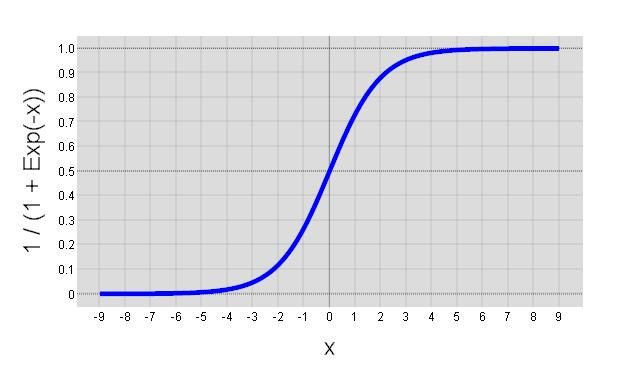
\includegraphics[width=0.5\linewidth]{figures/plots/sigmoid}}
\caption{This transformation is
  called the sigmoid function because the way it transforms all inputs into
  values makes it look like an ``S'' shape, with 0 outputs to the left,
  increasing in the middle (an input of 0 right at the threshold gives an
  output of 0.5) and 1 outputs to the right.}
\label{fig:watson:sigmoid}
\end{figure}

For this, we are going to need an \emph{objective function}: a mathematical
expression that tells us how far we are from our goal.
%
In this case our objective is to make the probability saying we should
buzz---computed from our weights---for incorrect buzzes be as low as possible.
%
So this means that we're going to transform our weights into a
probability~$\pi_i$ between zero and one that gets big when the weights pass the threshold:
%
\begin{equation}
  \pi_i = \sigma \left( \sum_j w_{j} x_{i,j} - b \right) \equiv p(\mbox{buzz} \g {\bm x}) \equiv \frac{1}{1+\exp{-\left(\sum_{j} w_j
        x_{i,j} + b \right)}}.
  \label{eq:watson:pi}
\end{equation}
%
Since we only want to buzz when we're right, then we want $\pi_i$ to be small
(close to zero) whenever the buzz is wrong and big when the buzz is right
(close to one).
%
Alternatively, we could also say we want $1-\pi_i$ to be big when the buzz is
wrong, since this means that $\pi_i$ is as close to zero.
%
This alternate formulation is actually what we want since we will want to
optimize a single function going in the same direction.
%
Because we care about all examples, you would normally multiply the
probability of joint events together, but this leads to a very small number
(since probabilities are less than one), so for mathematical convenience we
take the log:
\begin{equation}
  \mathcal{L}' \equiv = \explain{How right are we}{\sum_{i \in \mathcal{X}_c}
    \log{\pi_i}} + \explain{How wrong are we}{\sum_{i \in
      \mathcal{X}_f} \log{1 - \pi_i}}.
  \label{eq:watson:logprob}
\end{equation}
So this overall expression (the log probability) tells us how good of a job
our features are doing in telling us when to buzz.

Later in the book, objective functions like this will be called a \emph{loss
  function}, so to be consistent with that, we will think about how to
\emph{minimize our mistakes}, so what we will do now (somewhat confusingly) is
to minimize the negative of $\mathcal{L}'$, which we will call $\mathcal{L}$:
\begin{equation}
  \mathcal{L} \equiv = -\sum_{i \in \mathcal{X}_c}
    \log{\pi_i}} - \sum_{i \in
    \mathcal{X}_f} \log{1 - \pi_i}.
  \label{eq:watson:loss}
\end{equation}
Just to recap: Equation~\ref{eq:watson:pi} is the probability of the model
saying we should buzz on example~$i$, Equation~\ref{eq:watson:logprob}
combines all of those together to see how close we are to being right, and
then Equation~\ref{eq:watson:loss} flips it around so that the large it is,
the wronger we are\dots we want to minimize that expression.

If you remember high school calculus, this is an optimization problem: you can
compute the derivative (gradient, actually) of each of each of the variables
you have control over---the feature weights {\bm w}---and then adjust those
weights to decrease the loss function represented by $\mathcal{L}$
(Equation~\ref{eq:watson:loss}).
%
When you did this in high school calculus, you could probably solve the
equation for when the derivative was zero, set the variable to make the
derivative zero, and then you're done.
%
But that's not possible here, so we need to take little adjustments to ${\bm
  w}$ to push $\mathcal{L}$ down again and again.

An intuitive way of thinking about this is that the shape of $\mathcal{L}$
represents a hill.
%
Where you stand on the hill is represented by how you've set ${\bm w}$: each
dimension represents one dimension of this vector.\footnote{The threshold $b$
  is also an additional dimension you need to optimize, but we'll gloss over
  this for now\dots you can always fudge it be imagining it an additional
  dimension of {\bm w} that's always active for every example.}
%
In two dimensions, one dimension is how far north--south you are and one
dimension is how far east--west you are: and you're trying to get to the
lowest valley you can.
%
The catch is that you can't really see what the whole landscape looks like;
it's so foggy you can only see right around where you are.
%
The intuition in this case is to walk ``downhill'', and this is exactly what
the gradient of $\mathcal{L}$ gives you.

Now the problem is that computing $\mathcal{L}$ over your entire dataset is
hard: you have to go over every single question in the \jeopardy{} training
set to compute its contribution to the gradient.
%
The way that I like to think about it is that each example is a person you can
ask ``how do I go downhill''.
%
While you could ask lots of different people, if you ask literally everyone,
that's probably going to be overkill.
%
You can probably get a good sense of the direction by just asking a handful of
example of which way you should go.

In the lingo, the sample of examples that you ask for the direction is the
\emph{minibatch}, and this overall process of asking a few (or even one)
example for a direction is called \emph{stochastic gradient descent} as
invented by Leon\footnote{Fun fact: Leon was a researcher at \texttt{nec} next
  to Princeton when I defended my dissertation, and he came to my defense\dots
  I assume for the free food rather than for the content.} Bouttou~\citep{}.

Given that the math for the derivation is everywhere, I will skip it here (you
can take a look at Chapter XXXX of Speech and Language Processing by Jurafsky
and Martin, which I often use in my classes and thus have adopted their
notation), but it is so intuitive that if you look at it, it just ``feels
right''.
%
For a minibatch of size one, if you ask it which way you should go, it tells
you to update your weights ${\bm w}$ to be:
\begin{equation}
  {\bm w}^{\mbox{new}} = {\bm w}.
  \label{eq:watson:update}
\end{equation}
In other words, if you got this example right, you slightly increase all of
the feature weights that caused you to get it right.
%
If you got it wrong, you slightly decrease all of the feature weights that
caused you to get it wrong.

\jbgcomment{need to add a category}

For example, let's say that you have a clue
\question{XXXX}
that Watson famously got wrong as a final \jeopardy{} when it answered the
famous American city \answer{Toronto}.
%
So in this case our buzzer input\footnote{In reality, the calculus for Final
  \jeopardy{} is a little different because it makes sense to provide some
  answer no matter what, you don't really buzz in.  However, you still want
  the best answer to have the highest probability, so we can still work
  through this example.  And indeed, given the debugging output \watson{}
  showed it didn't seem very confident in its wrong output, so it probably
  wouldn't have ``buzzed in'' during normal play (but again, it's strategic to
  put something down), which suggests that everything was working as intended.
  The bigger complication is how to figure out what to wager going into the
  final given your opponents and the category, which we talk about at a
  cursory level in Section~\ref{sec:watson:wagers}.} is whether we should buzz
on this clue with the response \answer{Toronto}, for which we get a $\pi_i$.
%
For the sake of concreteness, let's say $\pi_i$ is 0.4\dots it's not high, but it
\emph{should} be zero because Midway and O'Hare airports are actually in
the great city of \answer{Chicago}.
%
Now this is too high, so something went wrong with our features.
%
Let's see what features were on and what their current weights
in Table~\ref{table:watson:features}.\footnote{Lest there be any doubt, I am making up these weights and
  features for a simple example\dots \watson{} had many more and better
  features.  And you normally don't have feature weights with such round numbers.}

\begin{tabular}
  \toprule
  Feature & Weight & $x_i$ \\
  \midrule
  \abr{ir} Score & 2 & 0.1 \\
  \underline{Toronto} compatability with Category & 1 & 0.2 \\
  Knowledge Base (\# Airports in Toronto) & 0.1 & 2 \\
  Previous responses (\answer{Toronto}) & 0.005 & 40 \\
  \midrule
  Bias & -0.1  &  \\
  \bottomrule
\end{tabular}

Next things to write:
- What pi is and why
- What the new weight is

Write somewhere:
- Things backprop cannot do (e.g., which features you have, how they're
computed ... e.g., might have interpreted US = American = continent), how it relates to feature representation

\subsection{Learning as You Go}
\label{sec:watson:updates}

Something that is particularly unique to Jeopardy! and not to the
other QA settings we’ve looked at is that the category is a huge
constraint on what the correct responses are.
%
A large part of the
Jeopardy! buzzer is figuring out the ``lexical answer type'': what kind of
thing can the answer be.
%
Part of
this is is looking at clues in the clue.
%
This chapter has used a lot of example clues like ``this woman'' (Sue
Grafton), ``this code breaker'' (Turing), ``this position'' (goaltender), or
``this group'' (Gilbert Islands).
%
These are hints about what kind of response is being sought.
%
And lest you think this is an artifice of the skilled writers of \jeopardy{},
this also appears in more ``natural'' questions like those people ask Google
(Chapter~\ref{chapter:nq}).

And part of what made Watson a good \jeopardy{} Player is that it would learn
as it explored the category.
%
After getting a couple of months wrong, Watson
can learn that all of the answers should be a month.
%
And this can be encoded as a binary feature: all of the previous answers in the
current category have been a $X$ (Month, President, City, etc.) and so is the
current guess.

One thing that made Watson particularly impressive was that it not just computed raw accuracy but also compared against human performance.  

This chart showed how Watson progressed in different iterations of the system, inching up to the cloud of Jeopardy! champions.  Ken Jennings is in red there, still clearly dominating even the final version of Watson.

\section{This Game is Rigged, I Tell Ya!}

These successes have been well documented (not least by \abr{ibm}
itself, who rightly celebrated the great achievements); however,
things were not perfect\dots the game was rigged.
%
It's useful to go over the lifecycle of an entire question: how it was
written, how it's communicated, how players answer, and how the game
unfolds afterward.
%
At every stage, there's a slight benefit to the computer, which taken
together makes this an unfair competition.

This is a problem!  First, it's a problem scientifically because we
want to have fair comparisons of human vs. computer intelligence.
%
More importantly, I want to have my turn having my question answering
robots face off against trivia whizzes (Chapter~\ref{ch:game-show}),
and I can't do that if everybody thinks that Watson's spin
on \jeopardy{} settled the issue (and it hasn't).

% Cite / read this:
% https://dominoweb.draco.res.ibm.com/reports/rc25356.pdf

But first, in case you don't know how \jeopardy{} works, we'll review
that.
%
However, if you've calculated a Coryat score before, you can go ahead
and skip ahead.


\subsection{The Pool of Questions}

\jbgcomment{Citation needed}

Part of the agreement between \jeopardy{} and \abr{ibm} was that the
competition would take place on normal, written questions.
%
In the media coverage of the competition, this focused on avoiding
video and picture daily doubles (fairly reasonable, but we'll discuss
this more in a bit).
%
However, this causes two problems: the questions are too easy and do
not necessarily challenge computers.

So what makes up ``normal'' questions?
%
Every game of \jeopardy{} has questions that range in difficulty.
%
Because it's a television show, many questions are easy enough that
the average viewer at home can get them.
%
Moreover, the humans on the stage with Watson are not normal contestants.
%
Ken Jennings is certifiably the greatest of all
time~\citep[\abr{goat}]{low-20} \jeopardy{} player, and Brad Rutter
isn't bad himself.

The average ``normal'' \jeopardy{} contestant, including not so great
players like yours truly, know a large majority of the clues.
%
For top players like Brad and Ken, they know---with a handful of
exceptions--\emph{all} the clues.
%
In a one-on-one fight with normal clues, Ken and Brad would be
fighting over every clue: it would come down to who could buzz first.

This isn't fun to play.
%
Nor is it fun to watch.
%
This is why \jeopardyp{}'s tournament of champions is played on much
more difficult clues~\citep{harris-06}.
%
Nonetheless, this is the battlefield where Watson won: ``normal''
questions that didn't challenge the human players.
%
Instead, it all came down to the buzzer.

\subsection{John Henry vs. the Buzzing Machine}

Unlike \qb{} (Chapter~\ref{ch:qb}), while \jeopardy{} also uses
signaling devices, these only work \emph{once the question has been
  read in its entirety}; Ken Jennings (also a former \qb{} player while he was a student at
\abr{byu}) himself explains it on a \textit{Planet Money}
interview~\citep{malone-19}:
\begin{quote}
{\bf Jennings:} The buzzer is
    not live until Alex finishes reading the question. And if you buzz
    in before your buzzer goes live, \emph{you actually lock yourself out
    for a fraction of a second}. So the big mistake on the show is
    people who are all adrenalized and are buzzing too quickly, too
    eagerly. \\
{\bf Malone:} \abr{ok}. To some degree, \jeopardy{} is kind of a video game, and a \emph{crappy video game where it's, like, light goes on, press button}---that's it. \\
{\bf Jennings:} (Laughter) Yeah. \\
\end{quote}
\jeopardy{}'s buzzers are a gimmick to ensure good television; however, \qb{} buzzers discriminate knowledge.

So how does this interact with Watson?
%
Watson receives all of the clues electronically and likewise gets an electronic signal to know when it is safe to buzz in.
%
In contrast, humans have to either guess when it is safe to buzz or
wait for a light to turn on.

\jbgcomment{citation needed for gurus}

\jeopardy{} gurus explicitly advise new players not to wait for the light---your puny human reflexes are too slow.
%
Indeed, one of Ken Jenning's strengths was his uncanny ability to
internalize the cadence of Alex's voice and when a technitian would
activate the buzzer~\citep{jennings-06}.
%
In contrast, Watson is literally an electromechanical buzzing machine
that could get first crack at every question it wants.\footnote{In
practice, this is not always true.  Because Watson computed its
responses in real time, it could not come up with a response in time
for particularly short questions.}

Unfortunately, despite subjecting everyone within earshot to these
rants, the computer science community thinks that the question is
settled: computers are better than humans at answering questions.
%
This is despite Ken basically saying that it did, indeed, come down to
the buzzer.

Moreover, what makes for a ``normal'' difficulty question for a human
does not always apply to a computer.
%
Let's first talk about what makes a clue easier for a computer and
then we'll talk about what makes a clue harder for a computer.

\paragraph{Easy for a Computer.}

When I appeared on \jeopardyp{}, my final \jeopardy{} was:
\question{ After this woman's death, her daughter wrote, ``As far as we
  in the family are concerned, the alphabet now ends at Y''}
%
All of us got the question right; it just so happened that \jeopardy{}
used a very similar clue that aired as we were recording:
%
\question{``G'' is for grand master as well as this woman who received the 2009 Grand Master Award.}
%
The correct response is of course \answer{Sue Grafton}.
%
For poorly read contestant like myself, only studying previous clues
allowed us to get the answer right.
%
I've never read a Grafton book, but I know she writes mystery books and
has titles of the form \textit{``A'' is for Alibi} (and that's the
only title I can think without looking at Wikipedia).

For Watson, this is ``memorization'' is trivial: a single letter
implies that the answer is \underline{Grafton}.
%
But just like you should not think that I'm smart for getting lucky to
have seen a reused clue, you should not praise Watson for finding
near-repeat questions.
%
And it's not just trivia games: Google's dataset of questions (which
we'll talk about in more detail the next chapter) have
many identical questions~\citep{lewis-21}.
%
Moreover, Watson can also store the entirety of Wikipedia, easily
looking up capitals, authors, etc.

Indeed, when a computer can find \emph{an exact quote} (as was in my
final \jeopardy{} clue), the question becomes even easier.
%
Then the computer just needs to find the appropriate article that
contains the quote and then just find whatever entity is mostly likely
to be a \jeopardyp{} answer.

Where systems like Watson struggle are on computation, matching novels
and movies to plots, combining multiple clues, lateral thinking, and
wordplay~\citep{kaushik-18}.
%
And this is not just a matter of degree: computers struggle with \emph{all}
such questions, even if they're in the top row of \jeopardyp{}.
%
While a computer is theoretically good at math, the kinds of programs
that answer trivia questions struggle answering match questions with
numbers in the double digits~\citep{wallace-19:numbers}.

This is why the goal of \abr{ai} is \emph{general} artificial
intelligence (Chapter~\ref{ch:turing}): while we can build specialized
systems for \jeopardy{} questions or math questions, unlike a
reasonably smart human, a single program can't ``do it all''.
%
Unlike for human contestants, the ``difficulty'' of \jeopardy{}
questions for a computer has no relationship to the nominal value.
%
We talk about how Facebook/Meta dealt with this problem in
Chapter~\ref{ch:dynabench}: tell the authors what's hard for a computer.


\subsection{Two Nice Guys, One Computer with no Shame}

Given the ``too easy'' questions and the buzzer, what does this
actually mean for gameplay?
%
A question comes in, and Watson has the choice of answering it or not:
it can win every race to the buzzer if it wants.
%
Then, of the things it cannot answer, Ken and Brad fight over the
scraps.
%
Thus, for a computer to win this competition, it needs only to be able
to answer a third of the questions correctly.

Now, the \jeopardy{} nerds reading the book (I love you all), will
point out that this isn't true, because the clues are not weighted
equally: some are worth more than others.
%
However, as we discussed above, what's difficult for a computer isn't
always difficult for a human (and \textit{vice versa}), so it really
is a random third of the questions.
%
While a good human player might be weak on the buzzer and be confident
that if they know more they'll win the harder clues, this isn't true
for a human facing off against Watson.

Moreover, the computer has no shame: it uses a strategy called the
``Forrest Bounce''~\citep[more infamously associated with James Holzhauer
and Arthur Chu]{rogak-20}.
%
Rather than going through the categories top to bottom (easy to hard),
Watson goes through the clues somewhat randomly, searching for Daily
Doubles and trying to optimize its score.
%
Again, there's nothing wrong with this---it's the optimal strategy!
%
But if it's the ``right'' way to play the game, why doesn't every
human do it?

That's because humans want to follow social norms.
%
The producers of the show (hi, Maggie and Corinna!) tell you up and
down that you shouldn't play the game like that, and you don't want to
make them unhappy with you\dots they can make your life miserable.
%
I remember watching \jeopardy{} with my grandmother and when someone
hunted for the Daily Double, she would always say ``who does he think
he is'' (and it was always a he).
%
Alex Trebek also wasn't a
fan~\citep{marchese-18}:\footnote{\citet{rogak-20} quotes a saltier
  take Trebek offered to Howard Stern: ``It only works, dickweed, if
  you know the correct response to everything that's up there.''}
%
\begin{quote}
  When the show's writers construct categories they do it so that
  there's a flow in terms of difficulty, and if you jump to the bottom
  of the category you may get a clue that would be easier to
  understand if you'd begun at the top of the category and saw how the
  clues worked. I like there to be order on the show, but as the
  impartial host I accept disorder.
\end{quote}
%
And nobody, nobody, wants to make Alex unhappy.

Ken would sometimes do a little hunding for the Daily Double against a
particularly formiddable opponent, but he would normally be
well-behavied so as not to upset the powers that be.
%
Watson, however, was a soulless machine; and having a machine on the
stage was no exciting that
nobody faulted it for its strategy.
%
If anyone is to blame, it's probably Gary Tesauro; adding his
strategy for playing the board increased Watson's win percentage
considerably~\citep{tesauro-13}.
%
But if you put him in a room with the withering stares of \jeopardy{}
producers (or worse, Alex Trebek) and that code would be deleted in no
time.

% TODO(jbg): Cut substantially

\section{The Legacy of Watson}

% TODO (jbg): Add good stuff --- Tesauro, LAT, retriever--reader pipeline

Let's review Watson's appearance on \jeopardyp{}:
\begin{enumerate*}
        \item all questions are of ``normal'' difficulty;
        \item thus the two human contestants know nearly all of the clues; but
        \item Watson can win the buzzer race whenever it wants.
\end{enumerate*}
If Watson wins such a match, does that mean that it is superior to
these supurb humans?

I hope that you are reluctant to answer ``yes'' (not just
because \jeopardy{} has trained you to respond to answers with
questions).
%
Perhaps I've planted a seed of doubt: \emph{no, we cannot yet conclude
  computer superiority} from this experiment.
%
While many might want to believe that Watson is the end of
human--computer question answering competitions, it's only the
beginning.
%
Watson was just the beginning of the story, a story that unfolds
further in the next few chapters.

While \jeopardy{} and quiz bowl are the domain of trivia nerds, what
happens when computer scientists set the stage to decide whether
humans or computers are smarter?
%
Do humands stand a chance on \emph{that} battlefield?
